\section{Path Style}

\subsection{样式概述}

在 path 中添加修饰是十分自由的,在路径的任意地点添加的全局修饰都将起到相同的效果,同一段路径也允许有多个修饰,以下语句的效果相同。

\begin{lstlisting}[style = latex-side]
    \path [draw,fill] (0,0) circle (1cm);
    \path [draw] [fill] (0,0) circle (1cm);
    \path [fill] (0,0) circle (1cm) [draw];
    \draw [fill] (0,0) circle (1cm);
    \fill (0,0) [draw] circle (1cm);
    \filldraw (0,0) circle (1cm);
\end{lstlisting}

下面指令都是基于 \textbackslash path 指令衍生出来的常用指令:
\begin{itemize}
    \item \textbackslash draw  
    
    等效于 \textbackslash path[draw];绘制边线。
    \item \textbackslash fill 
    
    等效于 \textbackslash path[fill];填充颜色。
    \item \textbackslash filldraw
    
    等效于 \textbackslash path[fill,draw];绘制边线并填充颜色。
    \item \textbackslash pattern  
    
    等效于 \textbackslash path[pattern];填充图案。
    \item \textbackslash shade  
    
    等效于 \textbackslash path[shade];产生投影。
    \item \textbackslash shadedraw  
    
    等效于 \textbackslash path[shadedraw];绘制边线与投影。
    \item \textbackslash clip  
    
    等效于 \textbackslash path[clip];切片?
    \item \textbackslash useasboundingbox  
    
    等效于 \textbackslash path[useasboundingbox];绘制边框。
\end{itemize}


路径具有多种修饰,且部分修饰的值可能会重复,例如 color,有 fill = <color>,draw = <color> 等,如果不指定修饰名(键)则默认全部相关修饰均采用。

\begin{figure}[H]
    \centering
    \begin{minipage}{0.35\linewidth}
        \centering
        
\begin{tikzpicture}[scale = 1]
            \path[yshift = 0cm, fill = red!20] (0,0) circle (1ex);
            \path[yshift = 2em, draw = red!20] (0,0) circle (1ex);
            \path[yshift = 4em, red!20,fill,draw] (0,0) circle (1ex);
        \end{tikzpicture}
    \end{minipage}
    \begin{minipage}{0.55\linewidth}
        \begin{lstlisting}[style = latex-side]
    
\begin{tikzpicture}[scale = 1]
        \path[yshift = 0cm, fill = red!20] (0,0) circle (1ex);
        \path[yshift = 2em, draw = red!20] (0,0) circle (1ex);
        \path[yshift = 4em, red!20,fill,draw] (0,0) circle (1ex);
    \end{tikzpicture}
        \end{lstlisting}
    \end{minipage}
    \caption{Path Style:color}
\end{figure}

\subsection{线条样式}
\subsubsection{线条粗细}

\begin{itemize}
    \item line width = <dimension> \hfill (默认:0.4pt)
    
    控制线条粗细,该键可以省略。

    \begin{figure}[H]
        \centering
        \begin{minipage}{0.35\linewidth}
            \centering
            
\begin{tikzpicture}[scale = 1]
                \draw[line width = 5pt] (0,0) -- (3,0);
            \end{tikzpicture}
        \end{minipage}
        \begin{minipage}{0.55\linewidth}
            \begin{lstlisting}[style = latex-side]
    \draw[line width = 5pt] (0,0) -- (3,0);
            \end{lstlisting}
        \end{minipage}
        \caption{Path Style:line width}
    \end{figure}

    TikZ 为我们预设了几种常用的粗细,它们的值如下:

    \begin{table}[H]
        \centering
        \caption{line width:预设值}
        \label{table:line width:预设值}
        \setlength{\tabcolsep}{5mm}
        \begin{tabular}{cc|cc|cc}
            \toprule
            \textbf{名称} & \textbf{粗细} & \textbf{名称} & \textbf{粗细} & \textbf{名称} & \textbf{粗细} \\
            \midrule
            ultra thin  & 0.1pt  & very thin & 0.2pt & thin & 0.4pt \\
            semithick   & 0.6pt  & thick     & 0.8pt & very thick & 1.2pt \\
            ultra thick   & 1.6pt  &&&& \\
            \bottomrule
        \end{tabular}
    \end{table}

    \begin{figure}[H]
        \centering
        \begin{minipage}{0.35\linewidth}
            \centering
            
\begin{tikzpicture}[scale = 1]
                \draw [yshift = 0,    ultra thin]   (0,0) -- (3,0);
                \draw [yshift = -1em, very thin]    (0,0) -- (3,0);
                \draw [yshift = -2em, thin]         (0,0) -- (3,0);
                \draw [yshift = -3em, semithick]    (0,0) -- (3,0);
                \draw [yshift = -4em, thick]        (0,0) -- (3,0);
                \draw [yshift = -5em, very thick]   (0,0) -- (3,0);
                \draw [yshift = -6em, ultra thick]  (0,0) -- (3,0);
            \end{tikzpicture}
        \end{minipage}
        \begin{minipage}{0.55\linewidth}
            \begin{lstlisting}[style = latex-side]
    \draw [yshift = 0,    ultra thin]   (0,0) -- (3,0);     % 0.1pt
    \draw [yshift = -1em, very thin]    (0,0) -- (3,0);     % 0.2pt
    \draw [yshift = -2em, thin]         (0,0) -- (3,0);     % 0.4pt
    \draw [yshift = -3em, semithick]    (0,0) -- (3,0);     % 0.6pt
    \draw [yshift = -4em, thick]        (0,0) -- (3,0);     % 0.8pt
    \draw [yshift = -5em, very thick]   (0,0) -- (3,0);     % 1.2pt
    \draw [yshift = -6em, ultra thick]  (0,0) -- (3,0);     % 1.6pt
            \end{lstlisting}
        \end{minipage}
        \caption{Path Style:线条粗细关键字}
    \end{figure}

\end{itemize}

\subsubsection{描边样式}
\begin{itemize}
    \item line cap = <type> \hfill (默认:butt)
    
    用于指明线条端点样式,有 round,rect,butt 三种样式:

    \begin{figure}[H]
        \centering
        \begin{minipage}{0.35\linewidth}
            \centering
            
\begin{tikzpicture}[scale = 1]
                \begin{scope}[line width=10pt]
                    \draw[line cap=round] (0,1 ) -- +(3,0);
                    \draw[line cap=butt] (0,.5) -- +(3,0);
                    \draw[line cap=rect] (0,0 ) -- +(3,0);
                \end{scope}
                \draw[white,line width=1pt]
                    (0,0 ) -- +(3,0) (0,.5) -- +(3,0) (0,1 ) -- +(3,0);
            \end{tikzpicture}
        \end{minipage}
        \begin{minipage}{0.55\linewidth}
            \begin{lstlisting}[style = latex-side]
    
\begin{tikzpicture}[scale = 1]
        \begin{scope}[line width=10pt]
            \draw[line cap=round] (0,1 ) -- +(3,0);
            \draw[line cap=butt] (0,.5) -- +(3,0);
            \draw[line cap=rect] (0,0 ) -- +(3,0);
        \end{scope}
        \draw[white,line width=1pt]
            (0,0 ) -- +(3,0) (0,.5) -- +(3,0) (0,1 ) -- +(3,0);
    \end{tikzpicture}
            \end{lstlisting}
        \end{minipage}
        \caption{Path Style:line cap}
    \end{figure}

    \item line join = <type> \hfill (默认:miter)
    
    用于指定线条拐角处的样式,有 round,bevel,miter 三种。

    \begin{figure}[H]
        \centering
        \begin{minipage}{0.35\linewidth}
            \centering
            \begin{tikzpicture}[scale = 1]
                \begin{tikzpicture}[line width=10pt]
                    \draw[line join=round] (0,0) -- ++(.5,1) -- ++(.5,-1);
                    \draw[line join=bevel] (1.25,0) -- ++(.5,1) -- ++(.5,-1);
                    \draw[line join=miter] (2.5,0) -- ++(.5,1) -- ++(.5,-1);
                    \useasboundingbox (0,1.5); % enlarge bounding box
                \end{tikzpicture}
            \end{tikzpicture}
        \end{minipage}
        \begin{minipage}{0.55\linewidth}
            \begin{lstlisting}[style = latex-side]
    
\begin{tikzpicture}[line width=10pt]
        \draw[line join=round] (0,0) -- ++(.5,1) -- ++(.5,-1);
        \draw[line join=bevel] (1.25,0) -- ++(.5,1) -- ++(.5,-1);
        \draw[line join=miter] (2.5,0) -- ++(.5,1) -- ++(.5,-1);
        \useasboundingbox (0,1.5); % enlarge bounding box
    \end{tikzpicture}
            \end{lstlisting}
        \end{minipage}
        \caption{Path Style:line join}
    \end{figure}

    \item miter limit = <factor>  \hfill (默认:10)
    
    当夹角过小时,拐角处往往会显得过尖,用 miter limit 可以限制这一情况。

    \begin{figure}[H]
        \centering
        \begin{minipage}{0.7\linewidth}
            \centering
            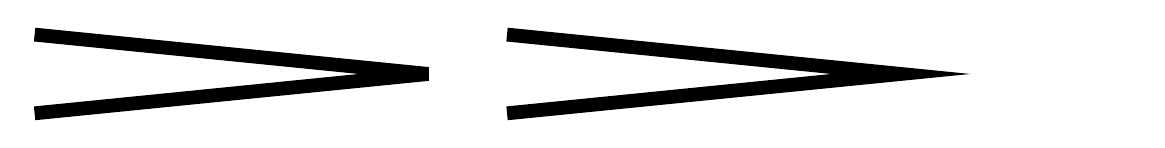
\begin{tikzpicture}[line width=5pt]
                \draw (0,0) -- ++(5,.5) -- ++(-5,.5);
                \draw[miter limit=25] (6,0) -- ++(5,.5) -- ++(-5,.5);
                \useasboundingbox (14,0); % make bounding box bigger
            \end{tikzpicture}
        \end{minipage}
        \begin{minipage}{0.7\linewidth}
            \begin{lstlisting}[style = latex-side]
    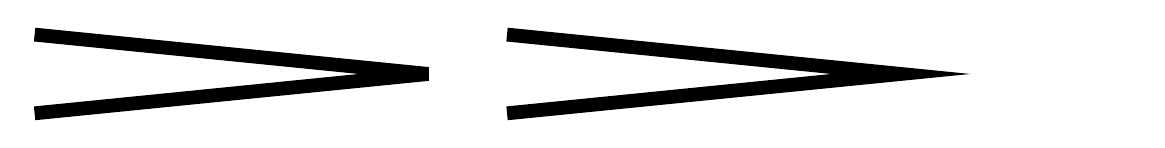
\begin{tikzpicture}[line width=5pt]
        \draw (0,0) -- ++(5,.5) -- ++(-5,.5);
        \draw[miter limit=25] (6,0) -- ++(5,.5) -- ++(-5,.5);
        \useasboundingbox (14,0); % make bounding box bigger
    \end{tikzpicture}
            \end{lstlisting}
        \end{minipage}
        \caption{Path Style:miter limit}
    \end{figure}

\end{itemize}

\subsubsection{虚线样式}

\begin{itemize}
    \item dash pattern = <dash pattern>
    
    设置虚线样式,值中有两个关键字 on 表示绘制,off 表示空缺。

    \begin{figure}[H]
        \centering
        \begin{minipage}{0.35\linewidth}
            \centering
            \begin{tikzpicture}[dash pattern=on 2pt off 3pt on 4pt off 4pt]
                \draw (0pt,0pt) -- (3.5cm,0pt);
            \end{tikzpicture}
        \end{minipage}
        \begin{minipage}{0.55\linewidth}
            \begin{lstlisting}[style = latex-side]
    \begin{tikzpicture}[dash pattern=on 2pt off 3pt on 4pt off 4pt]
        \draw (0pt,0pt) -- (3.5cm,0pt);
    \end{tikzpicture}
            \end{lstlisting}
        \end{minipage}
        \caption{Path Style:dash pattern}
    \end{figure}

    \item dash phase = <dash phase>
    
    设置线条的起始位置。

    \begin{figure}[H]
        \centering
        \begin{minipage}{0.35\linewidth}
            \centering
            \begin{tikzpicture}[dash pattern=on 20pt off 10pt]
                \draw[dash phase=0pt] (0pt,3pt) -- (3.5cm,3pt);
                \draw[dash phase=10pt] (0pt,0pt) -- (3.5cm,0pt);
            \end{tikzpicture}
        \end{minipage}
        \begin{minipage}{0.55\linewidth}
            \begin{lstlisting}[style = latex-side]
    \begin{tikzpicture}[dash pattern=on 20pt off 10pt]
        \draw[dash phase=0pt] (0pt,3pt) -- (3.5cm,3pt);
        \draw[dash phase=10pt] (0pt,0pt) -- (3.5cm,0pt);
    \end{tikzpicture}
            \end{lstlisting}
        \end{minipage}
        \caption{Path Style:dash phase}
    \end{figure}

    \item dash = <dash pattern> phase <dash phase>
    
    可以将上面两个修饰合并为一个。

    \begin{figure}[H]
        \centering
        \begin{minipage}{0.35\linewidth}
            \centering
            \begin{tikzpicture}[scale = 1]
                \begin{tikzpicture}
                    \draw [dash=on 20pt off 10pt phase 0pt] (0pt,3pt) -- (3.5cm,3pt);
                    \draw [dash=on 20pt off 10pt phase 10pt] (0pt,0pt) -- (3.5cm,0pt);
                \end{tikzpicture}
            \end{tikzpicture}
        \end{minipage}
        \begin{minipage}{0.55\linewidth}
            \begin{lstlisting}[style = latex-side]
    \begin{tikzpicture}
        \draw [dash=on 20pt off 10pt phase 0pt] (0pt,3pt) -- (3.5cm,3pt);
        \draw [dash=on 20pt off 10pt phase 10pt] (0pt,0pt) -- (3.5cm,0pt);
    \end{tikzpicture}
            \end{lstlisting}
        \end{minipage}
        \caption{Path Style:dash}
    \end{figure}

    \item dash expand off 
    
    当路径长度不是一个 on 与 off 的整数倍时,往往会出现被截断的线段,使用该修饰可以强制使用完整的线段,将 off 增长以填充多余的区域。需要加载 decorations 包。

    \begin{figure}[H]
        \centering
        \begin{minipage}{0.35\linewidth}
            \centering
            \begin{tikzpicture}[|-|, dash pattern=on 4pt off 2pt]
                \draw [dash expand off] (0pt,30pt) -- (26pt,30pt);
                \draw [dash expand off] (0pt,20pt) -- (24pt,20pt);
                \draw [dash expand off] (0pt,10pt) -- (22pt,10pt);
                \draw [dash expand off] (0pt, 0pt) -- (20pt, 0pt);
            \end{tikzpicture}
        \end{minipage}
        \begin{minipage}{0.55\linewidth}
            \begin{lstlisting}[style = latex-side]
    \begin{tikzpicture}[|-|, dash pattern=on 4pt off 2pt]
        \draw [dash expand off] (0pt,30pt) -- (26pt,30pt);
        \draw [dash expand off] (0pt,20pt) -- (24pt,20pt);
        \draw [dash expand off] (0pt,10pt) -- (22pt,10pt);
        \draw [dash expand off] (0pt, 0pt) -- (20pt, 0pt);
    \end{tikzpicture}
            \end{lstlisting}
        \end{minipage}
        \caption{Path Style:dash expand off}
    \end{figure}

    \item 预设样式
    
    与 line width 类似的,TikZ 为我们提供了多个预设的虚线样式。

    \begin{table}[H]
        \centering
        \caption{Path Style - 预设样式}
        \label{table:Path Style - 预设样式}
        \setlength{\tabcolsep}{6mm}
        \begin{tabular}{c|ccc}
            \toprule
            \textbf{名称} & \textbf{基础样式} & \textbf{密集样式} & \textbf{松散样式} \\
            \midrule
            点 & dotted & densely dotted & loosely dotted \\
            虚线 & dashed & densely dashed & loosely dashed  \\
            点线 & dash dot & densely dash dot & loosely dash dot \\
            线点点 & dash dot dot & densely dash dot dot & loosely dash dot dot \\
            \bottomrule
        \end{tabular}
    \end{table}

    \begin{figure}[H]
        \centering
        \begin{minipage}{0.3\linewidth}
            \centering
            \begin{tikzpicture}[scale = 1]
                \draw [yshift = 0,solid]                        (0,0) -- (3,0);
                
                \draw [yshift = -2em,dotted]                    (0,0) -- (3,0);
                \draw [yshift = -3em,densely dotted]            (0,0) -- (3,0);
                \draw [yshift = -4em,loosely dotted]            (0,0) -- (3,0);

                \draw [yshift = -6em,dashed]                    (0,0) -- (3,0);
                \draw [yshift = -7em,densely dashed]            (0,0) -- (3,0);
                \draw [yshift = -8em,loosely dashed]            (0,0) -- (3,0);

                \draw [yshift = -10em,dash dot]                 (0,0) -- (3,0);
                \draw [yshift = -11em,densely dash dot]         (0,0) -- (3,0);
                \draw [yshift = -12em,loosely dash dot]         (0,0) -- (3,0);

                \draw [yshift = -14em,dash dot dot]             (0,0) -- (3,0);
                \draw [yshift = -15em,densely dash dot dot]     (0,0) -- (3,0);
                \draw [yshift = -16em,loosely dash dot dot]     (0,0) -- (3,0);
            \end{tikzpicture}
        \end{minipage}
        \begin{minipage}{0.6\linewidth}
            \begin{lstlisting}[style = latex-side]
    \draw [yshift = 0,solid]                        (0,0) -- (3,0);
    % 点
    \draw [yshift = -2em,dotted]                    (0,0) -- (3,0);
    \draw [yshift = -3em,densely dotted]            (0,0) -- (3,0);
    \draw [yshift = -4em,loosely dotted]            (0,0) -- (3,0);
    % 虚线            
    \draw [yshift = -6em,dashed]                    (0,0) -- (3,0);
    \draw [yshift = -7em,densely dashed]            (0,0) -- (3,0);
    \draw [yshift = -8em,loosely dashed]            (0,0) -- (3,0);
    % 点线
    \draw [yshift = -10em,dash dot]                 (0,0) -- (3,0);
    \draw [yshift = -11em,densely dash dot]         (0,0) -- (3,0);
    \draw [yshift = -12em,loosely dash dot]         (0,0) -- (3,0);
    % 线点点
    \draw [yshift = -14em,dash dot dot]             (0,0) -- (3,0);
    \draw [yshift = -15em,densely dash dot dot]     (0,0) -- (3,0);
    \draw [yshift = -16em,loosely dash dot dot]     (0,0) -- (3,0);
            \end{lstlisting}
        \end{minipage}
        \caption{Path Style:预设样式}
    \end{figure}

\end{itemize}

\subsubsection{双线条}

\begin{itemize}
    \item double = <core color>
    
    该修饰下绘制的线条将拥有两条线,它的内部处理方式为:首先根据 double 修饰提供的颜色绘制一条路径(默认为白色),再在所绘制路径的两边绘制新的路径,颜色由 draw 修饰给出(默认为黑色)。

    \begin{figure}[H]
        \centering
        \begin{minipage}{0.35\linewidth}
            \centering
            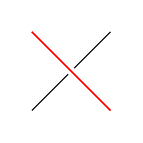
\begin{tikzpicture}[scale = 1]
                \draw (0,0) -- (1,1);
                \draw[draw=white,double=red,very thick] (0,1) -- (1,0);
            \end{tikzpicture}
        \end{minipage}
        \begin{minipage}{0.55\linewidth}
            \begin{lstlisting}[style = latex-side]
    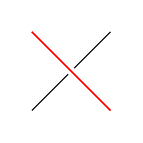
\begin{tikzpicture}[scale = 1]
        \draw (0,0) -- (1,1);
        \draw[draw=white,double=red,very thick] (0,1) -- (1,0);
    \end{tikzpicture}
            \end{lstlisting}
        \end{minipage}
        \caption{Path Style:double}
    \end{figure}

    \item double distance = <dimension> \hfill (默认:0.6pt)
    
    设置两条边线的距离。

    \begin{figure}[H]
        \centering
        \begin{minipage}{0.3\linewidth}
            \centering
            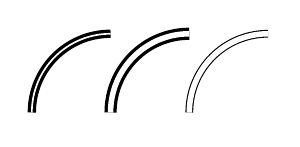
\begin{tikzpicture}[scale = 1]
                \draw[very thick,double] (0,0) arc (180:90:1cm);
                \draw[very thick,double distance=2pt] (1,0) arc (180:90:1cm);
                \draw[thin,double distance=2pt] (2,0) arc (180:90:1cm);
            \end{tikzpicture}
        \end{minipage}
        \begin{minipage}{0.6\linewidth}
            \begin{lstlisting}[style = latex-side]
    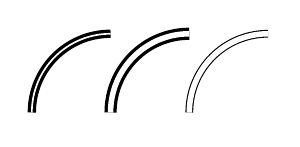
\begin{tikzpicture}[scale = 1]
        \draw[very thick,double] (0,0) arc (180:90:1cm);
        \draw[very thick,double distance=2pt] (1,0) arc (180:90:1cm);
        \draw[thin,double distance=2pt] (2,0) arc (180:90:1cm);
    \end{tikzpicture}
            \end{lstlisting}
        \end{minipage}
        \caption{Path Style:double distance}
    \end{figure}

    \item double distance between line centers = <dimension>
    
    该修饰与 double distance 类似,但它的距离计算是指两边线的中点的距离

    \begin{figure}[H]
        \centering
        \begin{minipage}{0.35\linewidth}
            \centering
            \begin{tikzpicture}[scale = 1]
                \begin{tikzpicture}
                    \foreach \lw in {0.5,1,1.5,2,2.5}
                        \draw[line width=\lw pt,double distance between line centers=3pt] (\lw,2em) -- ++(4mm,0);
                    \foreach \lw in {0.5,1,1.5,2,2.5}
                        \draw[line width=\lw pt,double distance = 3pt] (\lw,0) -- ++(4mm,0);
                \end{tikzpicture}
            \end{tikzpicture}
        \end{minipage}
        \begin{minipage}{0.55\linewidth}
            \begin{lstlisting}[style = latex-side]
    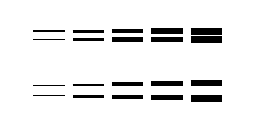
\begin{tikzpicture}
        \foreach \lw in {0.5,1,1.5,2,2.5}
            \draw[line width=\lw pt,double distance between line centers=3pt] (\lw,2em) -- ++(4mm,0);
        \foreach \lw in {0.5,1,1.5,2,2.5}
            \draw[line width=\lw pt,double distance = 3pt] (\lw,0) -- ++(4mm,0);
    \end{tikzpicture}
            \end{lstlisting}
        \end{minipage}
        \caption{Path Style:double distance between line centers}
    \end{figure}
    
\subsection{填充样式}






\end{itemize}






















\newpage